\documentclass[letterpaper, 12 pt, conference]{ieeeconf}  % Comment this line out
                                                          % if you need a4paper
%\documentclass[a4paper, 10pt, conference]{ieeeconf}      % Use this line for a4
                                                          % paper

\IEEEoverridecommandlockouts                              % This command is only
                                                          % needed if you want to
                                                          % use the \thanks command
\overrideIEEEmargins
\usepackage{listings}
\usepackage{amsmath}
\usepackage{algorithm}
\usepackage[noend]{algpseudocode}
\usepackage{gensymb}
\usepackage{graphicx}


\title{\LARGE \bf
Unstructured terrain navigation and  topographic mapping with a low-cost mobile cuboid robot
}

\begin{document}

\author
{Robert L. Baines$^{1}$, Andrew S. Morgan$^{1}$, Hayley McClintock$^{1}$,  and \\ Brian Scassellati $^{2}$ 
\thanks{$^{1}$Robert Baines, Andrew Morgan, and Hayley McClinktock are with the Department of Mechanical Engineering \& Materials Science, Yale University,  10 Hillhouse Avenue, New Haven, CT 06520, USA. (email: {\tt\small {Robert.Baines, Andrew.Morgan, Hayley.McClinktock}@yale.edu}).}
\thanks{$^{2}$Brian Scassellati is with the Department of Computer Science, Yale University,  51 Prospect Street, New Haven, CT 06511, USA. (email: {\tt\small {brain.scassellati}@yale.edu}).}
}


\maketitle
\thispagestyle{empty}
\pagestyle{empty}

%%%%%%%%%%%%%%%%%%%%%%%%%%%%%%%%%%%%%%%%%%%%%%%%%%%%%%%%%%%%%%%%%%%%%%%%%%%%
\begin{abstract}

Existing robotic terrain mapping techniques require expensive sensor suites, high memory data structures, and posit unrealistic assumptions about the nature of an environmental map. Here, we present a cube-shaped robot which can move through unstructured terrain and construct a topographic map of the surface that it traverses in real time, with low computational and sensor cost. Our approach devolves much of the task of mapping and locomotion to passive mechanical features. Movement is achieved by inflating silicone bladders on four of the robot's faces to destabilize the robot and topple the cube from face to face. Each of these faces contains arrays of fine plastic pins that conform to the geometry of terrain the robot rolls over. When the pins conform to the environment they rest upon, they displace inward into the cube. To reconstruct terrain contours and elevation from this mechanical displacement, a topography by shade algorithm is applied to capture images of the displaced pins. We then stitch together the images collected over the cube's trajectory to render detailed topographic maps in real-time. Our results show that this approach is viable for mapping unknown terrain in the robot's environment. 
\end{abstract}

%%%%%%%%%%%%%%%%%%%%%%%%%%%%%%%%%%%%%%%%%%%%%%%%%%%%%%%%%%%%%%%%%%%%%%%%%%%%
\section{INTRODUCTION}

The demand for increasingly autonomous robotic systems has motivated extensive research on ways robots can navigate and map environments. One common approach, simultaneous localization and mapping (SLAM), can reconstruct an environment in 3D and estimate robot pose in that environment by using a combination of sensory data acquired from on-board Lidar, cameras, GPS, or laser-based range finders \cite{SLAM_intro}. Although SLAM and its variants have been shown to depict obstacles and topography accurately, they construct environmental maps with high computational expense, limiting their applicability \cite{3D_mapping}. For instance, triangle meshes and raw data points are very accurate but require substantial memory \cite{triangle_mesh1}, \cite{triangle_mesh2}. Furthermore, many 3D reconstructions have constraints on the resolution of features they can map. Fine details are lost by virtue of the scales considered--typically large obstacles \cite{mapping_survey}. Additionally, most mapping algorithms and sensor infrastructure required to realize those algorithms are not transferable to unstructured environments, but rather well-defined corridors with flat surfaces \cite{mapping_survey}. Lastly, the suite of sensors required for accurate topographic reconstruction ramps up expense and complexity associated with building and deploying robots equipped with those sensors. 

% FIGURE 1: show schematic of the cuboid in action. Splash Figure
% Cover picture of constructed cuboid in front of obstacles.
 \begin{figure}
 \centering
 \includegraphics[width=0.5\textwidth]{Figures/Cuboid.png}
 \caption{Cuboid robot approaches obstacle course for topographical mapping with pin arrays and inflatable bladders exposed on the top and side. LED strips are strung throughout the cuboid to illuminate faces for the topography by shades approach. }
 \label{fig:operate} 
 \end{figure}
 
A compelling alternative to relying on optical and range sensor-driven mapping techniques and their high-dimensional data structures is to leverage tactile-based sensors to map an environment through direct physical interaction.  Minute or otherwise indistinguishable features and textures otherwise indiscernible for range-based systems could be tracked with tactile sensing with lower computational and monetary expense. For example, electro-active tactile sensors have been used in robotic hands to classify objects of diverse shapes and sizes \cite{tactile_robot_hand}. Deformation-based tactile sensors based on deforming fiducials on a compliant membrane \cite{tacile_sense_fiducial} or incident light changes \cite{tactile_sense_light} have been shown to elicit accurate surface and texture classifications under a variety of deformation conditions.  

We approach the challenge of creating navigating, mapping robots by relying on cheap, readily available materials for construction and minimizing the quantity and complexity of sensors. We propose to extend the traditional scope of tactile-based sensing by integrating arrays of displacement-based tactile sensors onto a mobile cuboid robot. 

In this work, we present a cuboid robot that can roll through varied terrain and construct accurate contour and elevation maps of the topography in real-time. Figure 1 depicts the cuboid robot in context of obstacle mapping. The cuboid robot moves by sequentially inflating two bladders on each of its four faces to locally destabilize itself and fall to a subsequent face. To sense and map the terrain over which it rolls, the robot utilizes a passive sensing mechanism: an array of plastic pins, which give an approximate elevation and contour of the object cuboid falls upon. On the inside of the cube, light is flashed on different sides of the pins while pictures are taken with a wide-angle camera. Our approach physically separates the "brains" of the sensor from the part which deforms, increasing its resilience. 

The outline of this paper is as follows: Section II describes the hardware and software systems used in the robot, Section III outlines three experiments we performed on the cuboid robot to appraise its efficacy, and finally, Section IV concludes the paper with a  discussion of future work. 

%%%%%%%%%%%%%%%%%%%%%%%%%%%%%%%%%%%%%%%%%%%%%%%%%%%%%%%%%%%%%%%%%%%%%%%%%%%%
\section{Systems of the cuboid robot}

\subsection{Hardware}

% FIGURE 2: Show exploded view of face of cuboid and highlight the key features. 
 \begin{figure*}
 \centering
 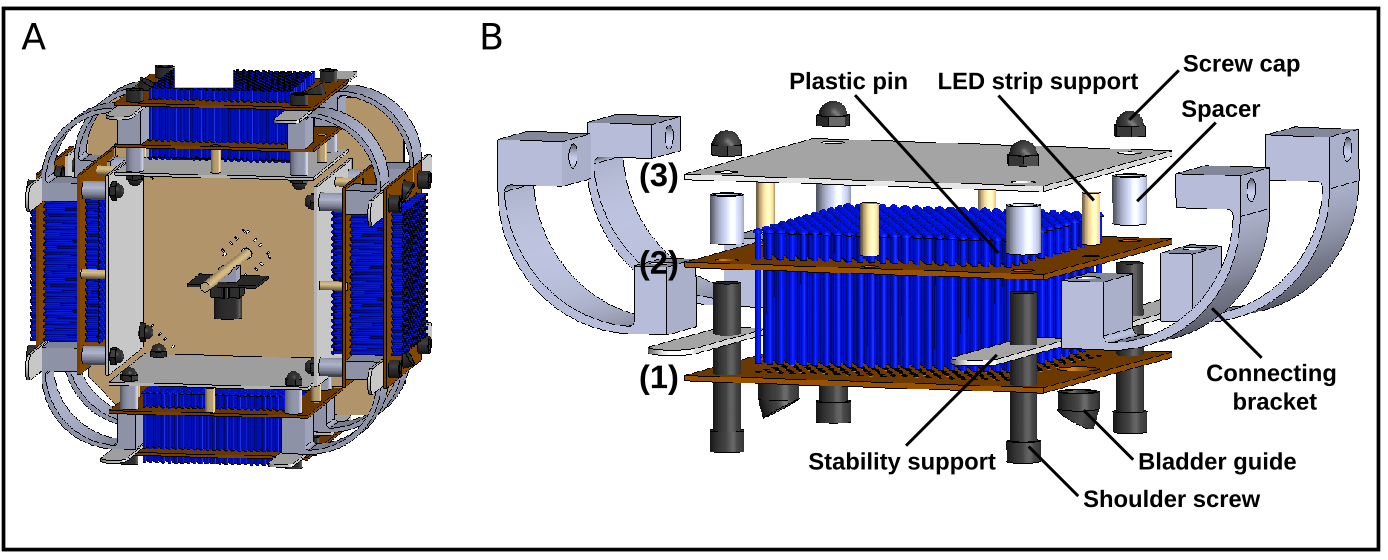
\includegraphics[width = 16cm]{Figures/explode.png}
 \caption{Schematic of the cuboid robot. (a) Open side view of the cuboid robot, including the camera and camera mounting system. (b) Exploded view of one face of the cuboid robot. Components are labeled and labels (1), (2), and (3) denote the outer, middle, and inner laser cut acrylic levels, respectively.}
 \label{fig:face} 
 \end{figure*}

The body of the cuboid robot is made primarily from sections of laser cut acrylic sheets (McMaster Carr) and custom 3D-printed connectors and brackets using a 3D printer (Prusa i3). Four of the six faces contain the sensing element: an array of plastic pins that are free to slide between two parallel acrylic plates. The two remaining faces are made from opaque acrylic, as to block out ambient light--blocking the light renders optimal conditions for the topography from shades algorithm--and contain holes for the camera mounting system and for routing wires and pneumatic lines out of the robot's interior to the off-board control station. 

An exploded view of one sensory face of the cuboid robot is shown in Figure 2. The face comprises three distinct levels. The first level (1)--the outermost with respect to the environment--contains the exposed pins. The pins are routed through small holes (1.35 mm diameter) so that they are free to translate vertically, but have minimal side-to-side movement. In addition, on the first level there are two bores where press-fit 3D printed inserts hold the pneumatic bladders. These inserts are angled so as to direct the inflation of the pneumatic bladder. The second level (2) is also cut with routing holes for the pins so as to provide a second constraint to prevent lateral movement. Additionally, four holes are added for press-fit \( \frac{1}{4} \) inch wooden dowels. These dowels route an addressable LED strip that is wrapped around the spacers between the second and third levels of the face. Finally, the third level (3) is made from a solid clear acrylic sheet, which prevents the pins from falling out when the face is rotated and provides a view of the pins for the camera to record. The three levels of the face are stacked and aligned using four plastic shoulder screws and 3D printed spacers. The spacers between levels one and two also serve as brackets that connect the four pin array faces together and are contoured to aid with rolling. Additional laser cut acrylic pieces are added between the spacer and level one acrylic to prevent the cuboid robot from rolling onto its non-sensing faces.

The camera mounting system on the cuboid robot consists of a \( \frac{1}{4} \) inch wooden dowel that is run between the two faces without pins. These faces are attached to the remaining four faces using magnets for easy access to the interior of the robot. The camera is attached to the wooden dowel with a 3D printed mount and zipties. This mounting system allows the camera to passively rotate with the robot during locomotion, relying on the force of gravity to reorient the lens towards the face of the robot contacting the ground. 

\subsection{Electronic infrastructure}

On board, the cuboid robot contains individually addressable LED strips (NooElec, WS2801) to illuminate the displaced pins and a wide-angle camera (ELP, megapixel Super Mini) to programmatically capture images. The power and data lines for the LED strip and camera are bound together and routed off board. The remaining electronic infrastructure is off board for the proof-of-concept prototype described in this paper. An array of 8 custom-made miniature pressure regulators \cite{p_regu} are used to control the inflation of the pneumatic bladders. The pressure regulators are addressable with a digital communication system based on the industry-standard I2C bus. 

Both the LEDs and the pressure regulators interface directly to the Arduino, which is in turn directed by the master controller via serial communications running on a PC. The camera is directly wired to the PC via a USB cable, which is processed by a vision processor node for topographical feature extraction and reconstruction.  

\subsection{Software architecture}

%FIGURE 3: insert ROS node or flow chart graphic. 
\begin{figure}
\centering
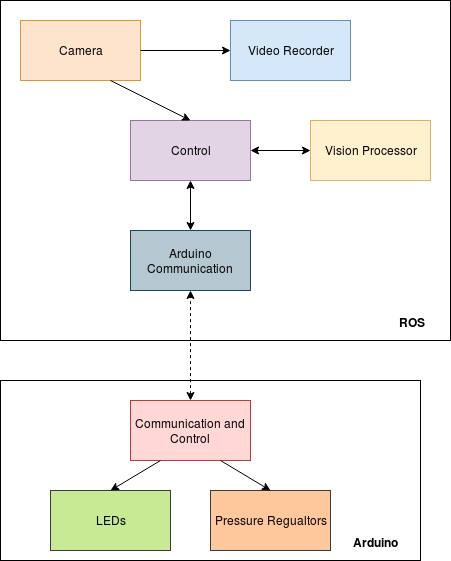
\includegraphics[width=0.5\textwidth]{Figures/Fig4.png}
\caption{The cuboid robot's software architecture comprises a collection of ROS nodes which interface via serial to an Arduino microcontroller, running the lower-level controls. On the ROS side, the control node receives current camera images, performs processing on the images, and saves the data. Upon completion, pre-specified commands are sent to the Arduino to activate rolling capabilities and lighting sequences. }
\label{fig:architecture_soft} 
\end{figure}

A master controller runs on a Linux PC with Robot Operating System (ROS) in order to coordinate a sequence of actions for the robot to perform. The ROS architecture is depicted in Figure 3. It contains five primary nodes, each with its own set of sub modules to execute robot-specific functionality. Low-level code running on the Arduino for the I2C bus and serial LED line is accessed by the master ROS controller. In the subsequent sections, each node in the software architecture is discussed in detail. 

\subsubsection{Camera node}

The camera node publishes raw images at a rate of 30Hz, which ensures up-to-date information used by the packages in processing. An optimal resolution of 640 x 480 pixels is found given the desired hardware to ensure high data throughput within the system. The sequence of RGB images are then easily distributed throughout the architecture to the video recorder node and the master control node, where data saving and processing will occur, respectively.   

\subsubsection{Control node}
The master controller coordinates sequential tasks within the ROS communication architecture by keeping a global clock and waiting for specific events to occur. The outline of this sequence is presented in Alg. 1. After rolling onto the desired cuboid face for mapping via \textit{inflateSequence(faceIt)} method, the controller specifies sequences of internal LED sections to be lit. This is a preprogrammed look-up table process in \textit{illuminateEdge()} to ensure desired LEDs are illuminated per face and per edge. During the illumination process the master controller records pictures from its camera subscription of the cuboid faces when each edge is illuminated. This process is completed for all edges (4) of the robot face. This data is then sent through the \textit{blurInterpolation()} method for further processing, as described in a following section. 

\makeatletter
\def\BState{\State\hskip-\ALG@thistlm}
\makeatother
\begin{algorithm}
\caption{Mapping Topography by Shades}\label{euclid}
\begin{algorithmic}[1]
	\renewcommand{\algorithmicrequire}{\textbf{Input:}}
	\renewcommand{\algorithmicensure}{\textbf{Output:}}
	\Require $begin$
	\Ensure $d_{face}$
    \State $faceIt$
    \Comment{Cuboid Face Iterator}
    \State $d_{face}$
    \Comment{Filtered Face Data}
    \While{$begin$}
      \State $inflateSequence(sideIt)$
      \Comment{Roll Cuboid}
      \For {$edge \in edges$}
         \State $illuminateEdge(edge)$ 
         \State $im[edge] \gets cuboidCamera()$
         \Comment{HSV}
         %\State $d_{edge}[edge] \gets processImage(im)$
      \EndFor
      \State $d_{face}[sideIt] \gets blurInterpolation(im)$
      \State $faceIt ++$
      \Comment{Increment Side}
      \EndWhile
     \State \Return $d_{face}$
\end{algorithmic}
\end{algorithm}


\subsubsection{Vision processor node and topography-by-shade algorithm}

The vision processing node receives and processes sequences of images provided from the camera node. Here, we implement the topography-by-shade algorithm. The algorithm for topographic map reconstruction of the displaced pins is inspired by the early computer vision technique "Shape from Shading", which initially used the 2D intensity map of an image to reconstruct its 3D geometry \cite{shape_shade}. In addition, the algorithm draws inspiration from another early computer vision technique from the late 80s, photometric stereo, which determines an object's surface orientation through incident illumination of the object over successive images, holding the viewing angle constant \cite{photometric}. Although current, more sophisticated photometric techniques exist for entire 3D surface reconstruction, such as accounting for arbitrarily positioned lights and multiple camera locations \cite{jin_2008}, our adaptation leverages assumptions of the aforementioned classical techniques to reduce computation time. 
 
 Like shape from shading, we assume that the reflected light intensity of an object is a function of its proximity to a viewing camera and the angle of the light source on the object. We do not consider the material reflectivity function and hold the position of the light source relative the the shape of interest constant. As in classical photometric stereo, we assume the image projection to the camera is orthographic (due to mechanical constraints in our system), and normals for some surface $z = f(x,y)$ are parameterized by a vector \cite{photometric}: 
 
 \begin{equation}
     [\frac{\partial f(x,y)}{\partial x}, \frac{\partial f(x,y)}{\partial y}, -1]
 \end{equation}
 
 To illuminate the displaced pins, we use four distinct light sources symmetrically located around the sensor area which cast equal intensities of light. This is accomplished by individually addressing sections of the continuous LED strands around the perimeter of the pins on each of the cuboid faces. We capture images of the displaced pins in each lighting condition, convert those images to hue saturation value (HSV) format, and average them. From the average image, we are able to easily extract a relative elevation profile because elevated areas are more illuminated in comparison to lower areas. 
 There are no significant constraints on our topography-from-shade method other than the final average image must be attained from symmetrically cast lights across the same area, and ambient light should not be overbearing (though our technique seems to perform reasonably even in well-lit office spaces). 

The algorithm for processing face images to a topographical map is summarized as follows: 

\makeatletter
\def\BState{\State\hskip-\ALG@thistlm}
\makeatother
\begin{algorithm}
\caption{blurInterpolation Method}\label{euclid}
\begin{algorithmic}[1]
	\renewcommand{\algorithmicrequire}{\textbf{Input:}}
	\renewcommand{\algorithmicensure}{\textbf{Output:}}
	\Require $im$
	\Ensure $d_{face}$
    \State $imAvg \gets averageImgs(im)$
    \Comment{Avg Data}
    \State $datBlur \gets blurNeighbors(imgAvg)$
    \State $datBlur \gets rmvPeakExtr(dataBlur)$
    \State $valleys \gets findValleys(datBlur)$
    \State $peaks \gets findPeaks(datBlur)$
    \State $d_{face} \gets interpolatePeaks(peaks,valleys)$
    \State \Return $d_{face}$
\end{algorithmic}
\end{algorithm}

\subsubsection{Arduino communication node} 

The Arduino communication node is responsible for creating a serial bridge between the Arduino and the ROS PC to facilitate communication. In this implementation, the Arduino listens for commands given from the master control node which signifies sections of the LED strips to turn ON/OFF, or pressure regulators to activate. While communication between the Arduino and the PC is bridged in order to transmit both directions, the implementation for this project is based off of an open-loop approach, which does not require sensing on the cuboid. Consequently, a one-way communication channel is used to give commands to the cuboid hardware in order to execute the desired task. 

%FIGURE 4: pictures and graph showing accuracy and lighting conditions over the objects. maybe table  
 \begin{figure}
 \centering
 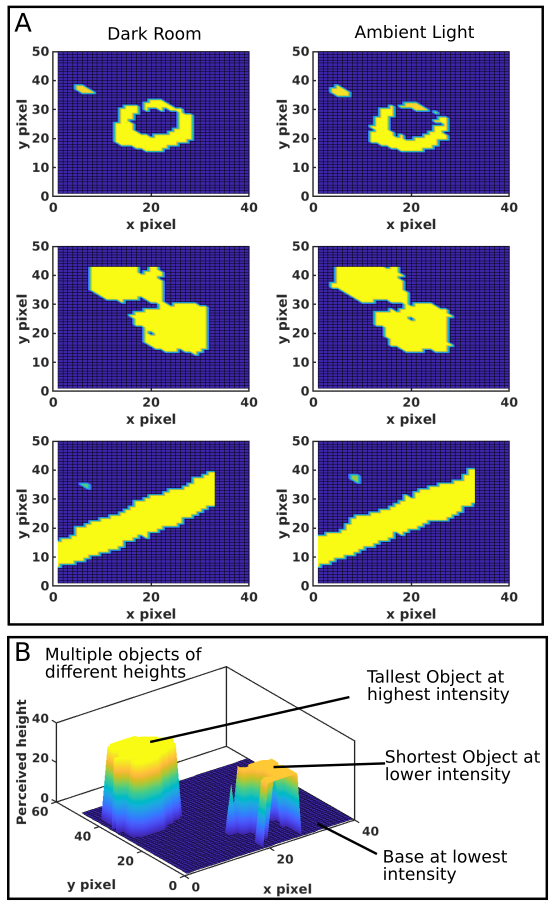
\includegraphics[width=0.48\textwidth]{Figures/Fig5.png}
 \caption{(A) sample of tested objects in the different lighting conditions. From top to bottom: nut, a pair of dice, and a mini screwdriver. Ambient light has minimal noticeable impact in the quality of the topographic reconstruction. (B) The algorithm is able to distinguish between multiple differently shaped objects of different heights and render clear, distinct entities, even in varying lighting conditions.}
 \label{fig:lighting} 
 \end{figure}

%%%%%%%%%%%%%%%%%%%%%%%%%%%%%%%%%%%%%%%%%%%%%%%%%%%%%%%%%%%%%%%%%%%%%%%%%%%%

%FIGURE 5: Graph of delta versus pressure and another graph of phi max the cube can roll up . 
\begin{figure*}
\centering
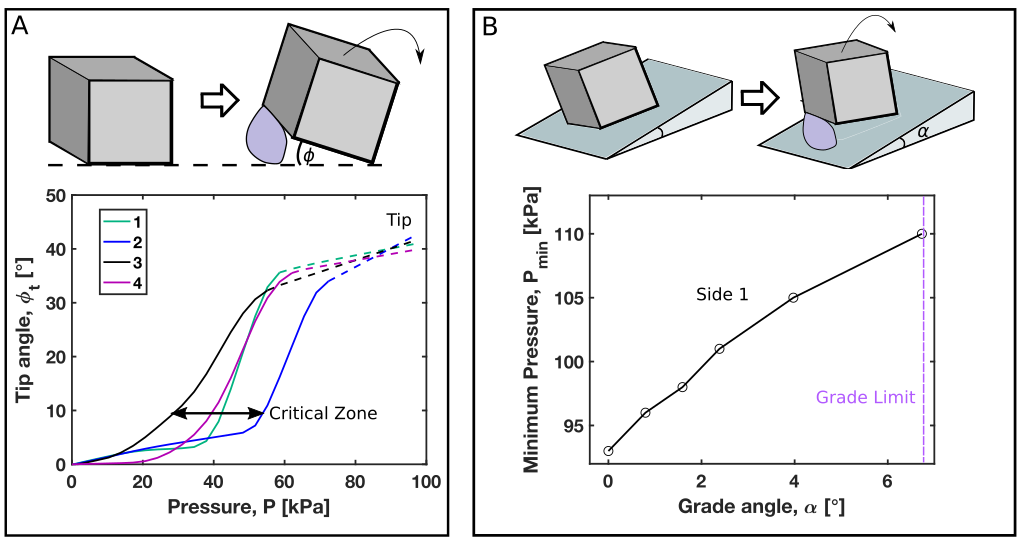
\includegraphics[width=0.9\textwidth]{Figures/Fig6.png}
\caption{(A) Pressure input versus the tip angle of the cuboid for all its faces. The cuboid experiences a quick rise in tip angle once a certain pressure has been passed. The secondary bladder activation denoted by the dashed part of the lines shows how only slightly more overall pressure needs to be input into the system to induce a roll. (B) The minimum pressure required to traverse sloped terrain of angle $\alpha$. We note }
\label{fig:tipping} 
\end{figure*}
\section{Testing and results}

We performed a number of tests on the cuboid robot to validate its efficacy.
\begin{enumerate}
    \item A test of the robustness of the simplified topography by shade approach to distinguish topographic features. Namely its capacity to distinguish topography accurately in two light conditions across differently shaped objects. 
    \item A characterization of the cube's pressure to tip angle relationship for moving across terrain, and the limitations, in terms of grade, that must be considered for successfully movement. 
    \item Validation of the full rolling cube system's efficacy in rolling and accurately rendering the topography over which it traversed.
\end{enumerate}

\subsection{Characterization of topography-by-shades algorithm}

We performed the topography-from-shading algorithm in two distinct lighting conditions to ascertain its transfer-ability to different environmental conditions. The first lighting condition was in total darkness, which we hypothesized would facilitate the most accurate reconstruction due to minimal external light noise sources. The second lighting condition was in ambient room lighting. In each lighting condition, three distinctly shaped were assessed: a ring-shaped nut, multiple dice, and a screwdriver, for a total of 6 independent tests. As a metric of accuracy, we appraised the reconstruction based on its ability to capture contours and continuous surfaces of the tested objects. 

Test results are conveyed visually in Figure 4A. The left column depicts results for the darkness condition, and the right, the ambient laboratory lighting condition. As predicted, the shape-by shades algorithm performed most accurately in total darkness, where only directional, controlled lighting patterns influenced topographic shading of the deformed pin array. Major differences are evident in the first example, the nut, in that the right upper-half of its top surface is less pronounced in ambient lighting. However, there was no marked differences observed between the lighting conditions for the other cases, suggesting our sensing and algorithmic approach is robust to various types of lighting. 

Figure 4B testifies to the algorithm's ability to segment objects of different heights correctly. This particular surface plot was rendered in ambient light. We found that the intensity of the LEDs drastically influenced correct contour and elevation segmentation; even more so than ambient lighting. The importance of considering internal, as well as external lighting in cuboid operation conditions is thus underscored. 

\subsection{Analysis of cuboid locomotion capabilities}

To test the cuboid robot's capability to navigate across varying terrain, we conducted an experiment to characterize how pressure input from the pneumatic actuators, $P$, correlated to the cuboid's angular displacement, $\phi$. The results are summarized in Figure 5A. Solid lines correspond to inflation of the first bladder on the cuboid. Dotted lines represent the second bladder. We considered cumulative input pressure, so the second bladder does not actually see upwards of 80kPa, but rather the end tipping pressure minus the maximum pressure attained by the first inflating bladder. According to Figure 5A, past a certain pressure threshold, the cube begins to tip at a fast rate for each increment in pressure. This property can be leveraged to tip the cube with less input pressure by increasing the flow rate of the pressure to the bladder and generating angular momentum about the cuboid's central axis. 

Another notable result evident in Figure 5A is the variance in pressure and tip angle for each of the sides of the cuboid. We attribute this variance to the relatively low quality of the commercially available silicone bladders used in the robot. The problem could be circumvented in future cuboid iterations by producing bladders via a standardized fabrication process to ensure their material properties and geometries remain consistent. On the software side, the problem could be remedied by using a PID controller to control their inflation, in lieu of simple bang-bang control. 

We then conducted an experiment to determine the maximum angle of inclines the cuboid robot could successfully roll up, and the corresponding minimum pressure required to traverse those inclines. Grade angles spanned from $\theta = 0\degree to 7\degree$. Figure 5B illustrates that the relationship between input pressure is approximately linear for the grade region in consideration. The cuboid fails to roll over once the grade exceeds around $7\percent$.  

\subsection{A robot obstacle course}

As a final assessment on the cuboid robot, we constructed an obstacle course, consisting of sequences of unique shapes emulating rocks, dirt, and other terrain. In particular, the course contained a metal cylindrical rod, several nuts, a wrench, a 3D-printed L-bracket, a small screwdriver, and a die. The metal rod and the nut were of the same vertical height. All other grouped objects were of disparate heights. We commanded the cuboid to roll across the simulated terrain and reconstruct a topographic map. We evaluated the reconstructed map based on ground truth images of the data and prior knowledge of their relative positions and elevations. 

Figure 6 showcases the actual topographic features (right) and those perceived by the cuboid robot (left). The middle image is the raw camera image of the deformed pin array. As a whole, the reconstruction qualitatively resembles the ground-truth objects fairly well. Contours are generally correct, as the reconstruction captures both internal and external geometric features like the center of the nut and the slot in the L-bracket. Distinct elevations (illustrated by the different colors of objects in the reconstruction map) were all identified successfully, save the second frame from top, in which the algorithm incorrectly put the small nut and wrench at the same elevation. We suspect this is the case because the objects did not have a large enough height difference to be segregated. 

\begin{figure}
\centering
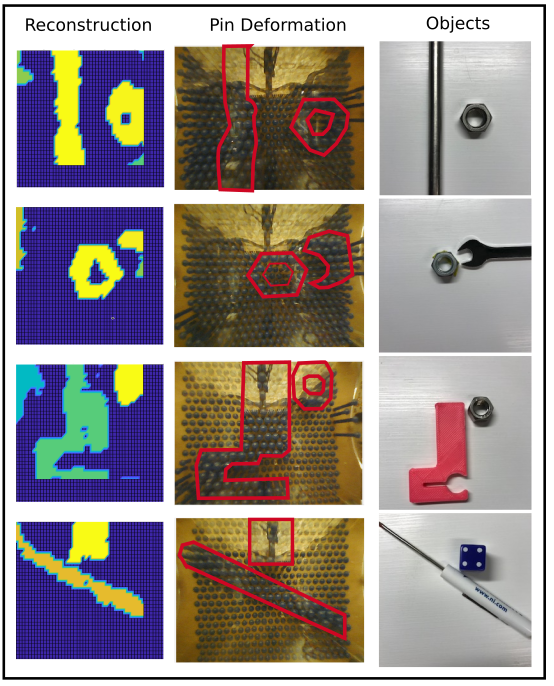
\includegraphics[width=0.49\textwidth]{Figures/Fig7.png}
\caption{Final mapped topography (left), pin deformation as captured inside the cube (middle), and ground-truth objects over which the cube rolled (right).}
\label{fig:obstacle course} 
\end{figure}

Marked deviation from ground-truth topography occurs about the periphery of the cuboid's captured image, probabaly resulting from glare from nearby LEDs. Additionally, some artifacts present in the reconstruction were the fault of the pin mechanism in that a few of its pins got stuck and persisted throughout the rolling duration, falsely indicating the presence of an object. Another issue was that the cuboid sensing face did not fall perfectly level to each object's surface, obfuscating the true contours of some objects. 

%%%%%%%%%%%%%%%%%%%%%%%%%%%%%%%%%%%%%%%%%%%%%%%%%%%%%%%%%%%%%%%%%%%%%%%%%%%%
\section{CONCLUSIONS}

This study presents a cuboid robot which simultaneously moves across and maps diverse terrains. The robot consists of commercially available, resilient, inexpensive components, and low-cost algorithms, in contrast with other mapping robots that utilize suites of complex sensors with computationally arduous SLAM. We envision that the presented design could be used to make swarms of robots that navigate and map in detail terrain where they are deployed. This capability would be particularly useful to automate land surveying on the massive-scale. The presented design also lends itself to extra-planetary exploration robotics and could autonomously map topography of planets and asteroids to identify resources. The concept is also transferable to fleets of robots which appraise field and soil conditions. 

The sensing apparatus and algorithms developed for the cuboid are transferable to larger scale robotic systems. We foresee that the tactile-based mapping strategy, topography-from-shade, will be a logical supplement to optical sensors for next-generation mobile robots, granting them heightened feature identification and reconstruction capabilities. 

%%%%%%%%%%%%%%%%%%%%%%%%%%%%%%%%%%%%%%%%%%%%%%%%%%%%%%%%%%%%%%%%%%%%%%%%%%%%

\addtolength{\textheight}{-12cm}   

%%%%%%%%%%%%%%%%%%%%%%%%%%%%%%%%%%%%%%%%%%%%%%%%%%%%%%%%%%%%%%%%%%%%%%%%%%%%

\section*{ACKNOWLEDGMENT}

Hayley McClintock was the chief designer of the robot's physical architecture, sensing, and actuation scheme. Andrew Morgan spearheaded the development of ROS node infrastructure, including the topography-from-shades algorithm. Robert Baines led the electronic system hardware and coding, and helped conceive the idea for the topography-from-shades algorithm.


The authors would like to thank Sarah Sebo for her dedication in handling myriad component orders from our team during the building process. This work was funded by the Department of Computer Science at Yale University. The class under which this project was carried out was CPSC 659, during the Fall Semester of 2018. The class was taught by Prof. Brian Scassellati. 


%%%%%%%%%%%%%%%%%%%%%%%%%%%%%%%%%%%%%%%%%%%%%%%%%%%%%%%%%%%%%%%%%%%%%%%%%%%%
\begin{thebibliography}{99}

\bibitem{SLAM_intro} M. Montemerlo, S. Thrun, D. Koller, and B. Wegbreit, “FastSLAM: A Factored Solution to the Simultaneous Localization and Mapping Problem,” p. 6.

\bibitem{triangle_mesh1} M. Levoy, K. Pulli, B. Curless, S. Rusinkiewicz, D. Koller, L. Pereira, M. Ginzton, S. Anderson, J. Davis, J. Ginsberg, J. Shade, and D. Fulk. The digital michelangelo project: 3D scanning of large statues. In Proc. SIGGRAPH, pages 131–144, 2000..

\bibitem{triangle_mesh2} C.F. Olson. Probabilistic self-localization for mobile robots. IEEE Transactions on Robotics and Automation, 16(1):55–66, 2000.

\bibitem{mapping_survey} S. Thrun, “Robotic Mapping: A Survey,” p. 31.

\bibitem{p_regu}J. W. Booth, J. C. Case, E. L. White, D. S. Shah, and R. Kramer-Bottiglio, “An addressable pneumatic regulator for distributed control of soft robots,” in 2018 IEEE International Conference on Soft Robotics (RoboSoft), Livorno, 2018, pp. 25–30.
%cite for pressure regulator 

\bibitem{shape_shade}B. K. P. Horn, “Obtaining Shape from Shading Information,” Psychology of Computer Vision. p. 42. 1975. 
% used to introduce concept of shape from shades 

\bibitem{jin_2008} H. Jin, D. Cremers, D. Wang, E. Prados, A. Yezzi, and S. Soatto, “3-D Reconstruction of Shaded Objects from Multiple Images Under Unknown Illumination,” International Journal of Computer Vision, vol. 76, no. 3, pp. 245–256, Mar. 2008.
%cite work that extended the photometric stereo to account for unkonwn light and multiple camera sources 
\bibitem{photometric} R. J. Woodham. "Photometric method for determining surface orientatoin from multiple images," Optical Engineering, vol. 19, no 1, pp. 139-144, Jan. 1980. 

\bibitem{finger_sense} Biomimetic and biohybrid systems: Second International Conference, Living Machines 2013, London, UK, July 29 - August 2, 2013. Proceedings, 1st edition. New York: Springer, 2013.

\bibitem{3D_mapping} R. Triebel, P. Pfaff, and W. Burgard, “Multi-Level Surface Maps for Outdoor Terrain Mapping and Loop Closing,” in 2006 IEEE/RSJ International Conference on Intelligent Robots and Systems, Beijing, China, 2006, pp. 2276–2282.
% justify that 3D mapping is computationally expenive 

\bibitem{tacile_sense_fiducial} A. Yamaguchi and C. G. Atkeson, “Optical Skin For Robots: Tactile Sensing And Whole-Body Vision,” RSS17 Workshop on Tactile Sensing for Manipulation: Hardware, Modeling, and Learning, Cambridge, MA, USA. p. 6.
%example of tactile sensing with deformed fiducials 

\bibitem{tactile_sense_light} B. McInroe, C. Chen, K. Goldberg, R. Bajcsy, and R. Fearing, “Towards a Soft Fingertip with Integrated Sensing and Actuation,” p. 8.

\bibitem{tactile_robot_hand} H. Yousef, M. Boukallel, and K. Althoefer, “Tactile sensing for dexterous in-hand manipulation in robotics—A review,” Sensors and Actuators A: Physical, vol. 167, no. 2, pp. 171–187, Jun. 2011.

\end{thebibliography}

\end{document}
